% =====================================================================
% Klausur-Cheatsheet Inferenzstatistik 1+2 -- 5 Seiten A4 quer, einseitig (final)
% =====================================================================
\documentclass[8pt,a4paper,landscape]{extarticle}

\usepackage[utf8]{inputenc}
\usepackage[margin=0.45cm]{geometry}
\usepackage{amsmath, amssymb}
\usepackage{multicol}
\usepackage[most]{tcolorbox}
\usepackage{enumitem}
\usepackage{xcolor}
\usepackage{array}
\usepackage{tabularx}
\usepackage{booktabs}
\usepackage{tikz}
\usepackage[expansion=false]{microtype}

\setlist{nosep, leftmargin=9pt, itemsep=0.4pt, topsep=0.6pt}
\setlength{\parindent}{0pt}
\setlength{\columnsep}{6pt}
\setlength{\parskip}{1pt}
\renewcommand\normalsize{\fontsize{8}{9.5}\selectfont}
\setlength{\tabcolsep}{2.5pt}
\renewcommand{\arraystretch}{1.12}
\pagestyle{empty}
\raggedcolumns
\sloppy

\definecolor{cWissen}{RGB}{27,84,150}
\definecolor{cRechnen}{RGB}{24,110,60}
\definecolor{cCode}{RGB}{70,70,70}
\definecolor{cFalle}{RGB}{170,30,30}

\tcbset{
  boxsep=0.4pt, left=2.2pt, right=2.2pt, top=1pt, bottom=1pt,
  boxrule=0.6pt, arc=1pt, enhanced, breakable,
  before skip=1.6pt, after skip=1.6pt,
  fonttitle=\bfseries\fontsize{8.5}{9.5}\selectfont,
  toptitle=0.7pt, bottomtitle=0.7pt,
}
\newtcolorbox{wissen}[1]{colback=cWissen!5,  colframe=cWissen,  coltitle=white, title={#1}}
\newtcolorbox{rechnen}[1]{colback=cRechnen!6, colframe=cRechnen, coltitle=white, title={#1}}
\newtcolorbox{werkzeug}[1]{colback=cCode!7,   colframe=cCode,    coltitle=white, title={#1}}
\newtcolorbox{falle}[1]{colback=cFalle!5,    colframe=cFalle,   coltitle=white, title={#1}}

\newcommand{\sect}[1]{\par\vspace{1pt}%
  {\fontsize{10}{11}\selectfont\bfseries #1}\par\nobreak\vspace{1pt}\nobreak}
\newcommand{\E}{\mathbb{E}}
\newcommand{\V}{\mathrm{Var}}
\newcommand{\Cov}{\mathrm{Cov}}
\newcommand{\iid}{\overset{iid}{\sim}}
\newcommand{\asim}{\overset{a}{\sim}}
\newcommand{\indep}{\mathrel{\perp\mkern-10mu\perp}}
\newcommand{\ra}{$\Rightarrow$}
\newcommand{\W}{\textbf{\textcolor{cRechnen}{W}}}
\newcommand{\F}{\textbf{\textcolor{cFalle}{F}}}
\newcommand{\ind}{\mathbf{1}}
% W/F-Tabelle: Aussage | W/F | Begründung
\newenvironment{wftab}{\renewcommand{\arraystretch}{1.02}\tabularx{\linewidth}{@{}>{\raggedright\arraybackslash}p{3.55cm}@{\hspace{3pt}}c@{\hspace{3pt}}>{\raggedright\arraybackslash}X@{}}}{\endtabularx}

% ---- Trace-Plot-Daten (Skizze auf Seite 4) ----
\newcommand{\traceKlein}[1]{\draw[#1] plot coordinates {(0.000,-0.293) (0.017,-0.287) (0.034,-0.294) (0.051,-0.325) (0.068,-0.339) (0.084,-0.335) (0.101,-0.340) (0.118,-0.340) (0.135,-0.332) (0.152,-0.317) (0.169,-0.317) (0.186,-0.308) (0.203,-0.311) (0.219,-0.281) (0.236,-0.285) (0.253,-0.299) (0.270,-0.285) (0.287,-0.283) (0.304,-0.283) (0.321,-0.283) (0.338,-0.279) (0.354,-0.286) (0.371,-0.286) (0.388,-0.264) (0.405,-0.261) (0.422,-0.264) (0.439,-0.255) (0.456,-0.258) (0.472,-0.254) (0.489,-0.244) (0.506,-0.244) (0.523,-0.244) (0.540,-0.244) (0.557,-0.233) (0.574,-0.233) (0.591,-0.228) (0.608,-0.203) (0.624,-0.197) (0.641,-0.175) (0.658,-0.181) (0.675,-0.155) (0.692,-0.143) (0.709,-0.138) (0.726,-0.150) (0.743,-0.129) (0.759,-0.138) (0.776,-0.135) (0.793,-0.154) (0.810,-0.154) (0.827,-0.142) (0.844,-0.147) (0.861,-0.151) (0.878,-0.163) (0.894,-0.165) (0.911,-0.162) (0.928,-0.138) (0.945,-0.170) (0.962,-0.180) (0.979,-0.180) (0.996,-0.163) (1.013,-0.178) (1.029,-0.177) (1.046,-0.146) (1.063,-0.134) (1.080,-0.106) (1.097,-0.085) (1.114,-0.088) (1.131,-0.064) (1.147,-0.069) (1.164,-0.061) (1.181,-0.076) (1.198,-0.038) (1.215,-0.046) (1.232,-0.067) (1.249,-0.054) (1.266,-0.049) (1.282,-0.046) (1.299,-0.051) (1.316,-0.049) (1.333,-0.056) (1.350,-0.062) (1.367,-0.068) (1.384,-0.055) (1.401,-0.029) (1.418,-0.015) (1.434,-0.013) (1.451,0.004) (1.468,0.006) (1.485,0.002) (1.502,0.014) (1.519,0.048) (1.536,0.082) (1.552,0.076) (1.569,0.087) (1.586,0.093) (1.603,0.118) (1.620,0.135) (1.637,0.120) (1.654,0.101) (1.671,0.117) (1.688,0.127) (1.704,0.131) (1.721,0.127) (1.738,0.139) (1.755,0.149) (1.772,0.167) (1.789,0.154) (1.806,0.145) (1.823,0.146) (1.839,0.143) (1.856,0.140) (1.873,0.137) (1.890,0.155) (1.907,0.124) (1.924,0.122) (1.941,0.131) (1.958,0.103) (1.974,0.101) (1.991,0.082) (2.008,0.093) (2.025,0.083) (2.042,0.074) (2.059,0.077) (2.076,0.065) (2.093,0.101) (2.109,0.103) (2.126,0.102) (2.143,0.094) (2.160,0.096) (2.177,0.078) (2.194,0.076) (2.211,0.061) (2.228,0.070) (2.244,0.082) (2.261,0.093) (2.278,0.106) (2.295,0.105) (2.312,0.125) (2.329,0.119) (2.346,0.149) (2.363,0.147) (2.379,0.166) (2.396,0.172) (2.413,0.159) (2.430,0.168) (2.447,0.171) (2.464,0.162) (2.481,0.148) (2.498,0.147) (2.514,0.148) (2.531,0.139) (2.548,0.121) (2.565,0.126) (2.582,0.100) (2.599,0.100) (2.616,0.115) (2.633,0.115) (2.649,0.095) (2.666,0.108) (2.683,0.117)};}
\newcommand{\traceGut}[1]{\draw[#1] plot coordinates {(0.000,-0.231) (0.017,-0.231) (0.034,-0.231) (0.051,-0.231) (0.068,-0.022) (0.084,-0.022) (0.101,-0.022) (0.118,0.089) (0.135,0.089) (0.152,0.089) (0.169,-0.103) (0.186,-0.103) (0.203,-0.103) (0.219,-0.040) (0.236,-0.004) (0.253,0.028) (0.270,0.028) (0.287,0.028) (0.304,-0.077) (0.321,0.153) (0.338,0.153) (0.354,0.153) (0.371,0.124) (0.388,-0.154) (0.405,-0.154) (0.422,-0.154) (0.439,-0.098) (0.456,0.110) (0.472,0.110) (0.489,0.110) (0.506,0.073) (0.523,-0.003) (0.540,-0.087) (0.557,0.094) (0.574,0.094) (0.591,0.094) (0.608,0.094) (0.624,0.094) (0.641,-0.025) (0.658,-0.025) (0.675,-0.025) (0.692,-0.072) (0.709,0.072) (0.726,0.072) (0.743,0.072) (0.759,0.072) (0.776,0.117) (0.793,0.117) (0.810,0.117) (0.827,0.117) (0.844,0.117) (0.861,0.010) (0.878,0.010) (0.894,-0.158) (0.911,0.160) (0.928,0.191) (0.945,0.191) (0.962,-0.138) (0.979,-0.099) (0.996,-0.099) (1.013,0.051) (1.029,0.051) (1.046,0.051) (1.063,0.051) (1.080,0.051) (1.097,-0.075) (1.114,-0.214) (1.131,-0.231) (1.147,0.098) (1.164,-0.049) (1.181,-0.049) (1.198,0.352) (1.215,0.303) (1.232,0.180) (1.249,0.180) (1.266,0.154) (1.282,0.154) (1.299,0.123) (1.316,0.123) (1.333,0.121) (1.350,0.121) (1.367,0.054) (1.384,0.054) (1.401,0.054) (1.418,0.054) (1.434,0.045) (1.451,-0.048) (1.468,-0.092) (1.485,0.028) (1.502,0.028) (1.519,0.028) (1.536,0.028) (1.552,0.028) (1.569,0.028) (1.586,0.028) (1.603,0.028) (1.620,-0.056) (1.637,-0.056) (1.654,-0.059) (1.671,-0.059) (1.688,-0.047) (1.704,-0.047) (1.721,-0.263) (1.738,-0.093) (1.755,-0.249) (1.772,-0.089) (1.789,0.011) (1.806,0.011) (1.823,-0.086) (1.839,0.006) (1.856,0.006) (1.873,0.006) (1.890,0.006) (1.907,0.006) (1.924,0.006) (1.941,0.006) (1.958,-0.115) (1.974,0.165) (1.991,0.048) (2.008,0.048) (2.025,0.048) (2.042,0.048) (2.059,0.048) (2.076,0.025) (2.093,0.025) (2.109,0.025) (2.126,0.025) (2.143,-0.043) (2.160,-0.043) (2.177,0.204) (2.194,0.327) (2.211,0.327) (2.228,0.327) (2.244,0.096) (2.261,-0.036) (2.278,-0.036) (2.295,-0.036) (2.312,-0.036) (2.329,-0.036) (2.346,0.203) (2.363,0.203) (2.379,-0.106) (2.396,-0.101) (2.413,-0.101) (2.430,-0.101) (2.447,-0.101) (2.464,-0.101) (2.481,-0.011) (2.498,-0.011) (2.514,-0.011) (2.531,-0.011) (2.548,0.095) (2.565,0.095) (2.582,0.095) (2.599,0.046) (2.616,0.046) (2.633,-0.153) (2.649,-0.195) (2.666,-0.195) (2.683,-0.029)};}
\newcommand{\traceGross}[1]{\draw[#1] plot coordinates {(0.000,-0.325) (0.017,0.152) (0.034,0.152) (0.051,0.152) (0.068,0.152) (0.084,0.152) (0.101,0.152) (0.118,0.152) (0.135,0.152) (0.152,-0.135) (0.169,-0.135) (0.186,-0.135) (0.203,-0.135) (0.219,-0.135) (0.236,-0.135) (0.253,-0.135) (0.270,-0.135) (0.287,-0.135) (0.304,-0.135) (0.321,-0.135) (0.338,-0.135) (0.354,-0.135) (0.371,-0.135) (0.388,-0.135) (0.405,-0.135) (0.422,0.004) (0.439,0.004) (0.456,-0.153) (0.472,-0.153) (0.489,-0.153) (0.506,-0.153) (0.523,-0.153) (0.540,-0.153) (0.557,-0.153) (0.574,-0.153) (0.591,-0.153) (0.608,-0.153) (0.624,-0.153) (0.641,-0.153) (0.658,-0.153) (0.675,-0.192) (0.692,-0.192) (0.709,-0.192) (0.726,-0.192) (0.743,-0.192) (0.759,-0.192) (0.776,0.054) (0.793,0.054) (0.810,0.054) (0.827,0.054) (0.844,0.054) (0.861,0.054) (0.878,0.054) (0.894,0.054) (0.911,0.054) (0.928,0.054) (0.945,0.065) (0.962,0.065) (0.979,0.065) (0.996,0.065) (1.013,0.065) (1.029,0.065) (1.046,0.065) (1.063,0.065) (1.080,0.065) (1.097,0.065) (1.114,0.065) (1.131,0.065) (1.147,0.065) (1.164,0.065) (1.181,0.065) (1.198,0.065) (1.215,0.065) (1.232,0.065) (1.249,0.065) (1.266,0.065) (1.282,0.065) (1.299,0.065) (1.316,0.065) (1.333,0.065) (1.350,0.065) (1.367,0.065) (1.384,0.065) (1.401,0.065) (1.418,0.065) (1.434,0.065) (1.451,0.065) (1.468,0.065) (1.485,0.065) (1.502,0.065) (1.519,0.065) (1.536,0.065) (1.552,0.160) (1.569,0.160) (1.586,0.160) (1.603,0.160) (1.620,0.160) (1.637,0.160) (1.654,0.160) (1.671,0.160) (1.688,0.160) (1.704,0.160) (1.721,0.160) (1.738,0.160) (1.755,0.081) (1.772,0.081) (1.789,0.081) (1.806,0.081) (1.823,0.081) (1.839,0.081) (1.856,0.081) (1.873,0.066) (1.890,0.066) (1.907,0.066) (1.924,0.066) (1.941,0.066) (1.958,0.066) (1.974,0.066) (1.991,0.066) (2.008,0.066) (2.025,0.066) (2.042,0.246) (2.059,0.246) (2.076,0.246) (2.093,0.246) (2.109,0.246) (2.126,0.299) (2.143,0.299) (2.160,0.299) (2.177,0.299) (2.194,0.299) (2.211,0.299) (2.228,0.299) (2.244,0.299) (2.261,0.299) (2.278,0.299) (2.295,0.299) (2.312,0.299) (2.329,0.299) (2.346,0.299) (2.363,0.299) (2.379,0.299) (2.396,0.299) (2.413,0.370) (2.430,0.370) (2.447,0.370) (2.464,0.370) (2.481,0.370) (2.498,0.370) (2.514,0.370) (2.531,0.315) (2.548,0.315) (2.565,0.315) (2.582,0.315) (2.599,0.315) (2.616,0.315) (2.633,0.315) (2.649,0.315) (2.666,0.315) (2.683,0.315)};}

\begin{document}
% ===================== SEITE 1: A1 Maximum Likelihood =====================
\begin{multicols*}{3}
\sect{A1 $\cdot$ Maximum Likelihood}
\begin{rechnen}{MLE-Rezept (jede Zeile = eigene Teilaufgabe)}
\begin{enumerate}[leftmargin=10pt]
\item \textbf{Likelihood:} $L(\theta)=\prod_{i=1}^n f(x_i;\theta)$. Hängt der Träger von $\theta$ ab: Indikator mitschreiben.
\item \textbf{Log-Likelihood:} $\ell(\theta)=\sum_{i=1}^n\log f(x_i;\theta)$. Summanden ohne $\theta$ (z.B.\ $n\log 3$) mit hinschreiben; sie fallen beim Ableiten weg.
\item \textbf{Score:} $s(\theta)=\frac{\partial\ell(\theta)}{\partial\theta}$ (nach $\theta$ ableiten, nicht nach $x$). $s(\theta)\overset{!}{=}0$ nach $\theta$ auflösen \ra{} $\hat\theta_{ML}$.
\item \textbf{Maximum zeigen:} $\ell''(\theta)<0$. Gilt es für alle $\theta$ \ra{} globales Maximum; sonst an der Stelle $\hat\theta$ prüfen.
\item \textbf{Fisher-Information:} $I(\theta)=-\E\big(\ell''(\theta)\big)=\V\big(s(\theta)\big)$. Erwartungswert von $\ell''$ bilden: jede Summe $\sum h(X_i)$ durch $n\cdot\E\big(h(X)\big)$ ersetzen (z.B.\ $\sum X_i^2\to n\,\E(X^2)$, nicht $n\,\E(X)^2$). Enthält $\ell''$ keine $X_i$: $I=-\ell''$. Bei iid: $I_n(\theta)=n\cdot I_1(\theta)$.
\item \textbf{Asymptotische Verteilung:} $\hat\theta_{ML}\asim N\big(\theta,\ I^{-1}(\theta)\big)$. Asymptotische Varianz $=I^{-1}(\theta)=\frac{1}{I(\theta)}$.
\item \textbf{Wald-KI:} $\hat\theta\pm z_{1-\alpha/2}\sqrt{I^{-1}(\hat\theta)}$ \ (in $I^{-1}$ wird $\theta$ durch $\hat\theta$ ersetzt).
\end{enumerate}
\end{rechnen}
\begin{falle}{Typische A1-Fehler}
\begin{itemize}
\item $\sum_{i=1}^n\log\theta=n\log\theta$ (Faktor $n$ nicht vergessen).
\item Maximum-Nachweis weglassen kostet Punkte.
\item In $I(\theta)$ keine $x_i$ stehen lassen: erst Erwartungswert bilden.
\item Varianz ist $I^{-1}$, nicht $I$. Asymptotische Verteilung mit wahrem $\theta$ angeben, im KI $\hat\theta$ einsetzen.
\item Wald-KI kann den Parameterraum verlassen (z.B.\ negative Grenze bei $\theta>0$).
\end{itemize}
\end{falle}
\begin{rechnen}{Konsistenz begründen: Definition + ein Weg}
\textbf{Definition:} $\hat\theta_n$ heißt (schwach) konsistent, wenn $P(|\hat\theta_n-\theta|>\varepsilon)\to 0$ für $n\to\infty$ und jedes $\varepsilon>0$.
\begin{enumerate}[leftmargin=10pt]
\item \textbf{MLE-Satz:} Unter Regularitätsbedingungen ist der ML-Schätzer konsistent. Kurz prüfen: Träger hängt nicht von $\theta$ ab, $f$ zweimal nach $\theta$ differenzierbar, $\theta$ im Inneren des Parameterraums. (Verletzt z.B.\ bei $U[0,\theta]$.)
\item \textbf{Über den MSE:} $\text{Bias}(\hat\theta)\to 0$ und $\V(\hat\theta)\to 0$ \ra{} $MSE\to 0$ (MSE-konsistent) \ra{} schwach konsistent (Tschebyscheff).
\item \textbf{GGZ:} Ist $\hat\theta$ eine stetige Funktion eines Mittelwerts $\frac1n\sum g(X_i)$: dieser konvergiert gegen $\E\big(g(X)\big)$ (Gesetz der großen Zahlen), also konvergiert auch $\hat\theta$ (stetige Abbildung).
\end{enumerate}
\end{rechnen}
\begin{rechnen}{Transformierter Parameter $\gamma=g(\theta)$}
\textbf{MLE von $\gamma$ (Invarianz):} $\hat\gamma_{ML}=g(\hat\theta_{ML})$. Einfach einsetzen, nichts neu ableiten.
\textbf{Verteilung (Delta-Methode):}
$$\hat\gamma\asim N\Big(g(\theta),\ g'(\theta)^2\cdot I^{-1}(\theta)\Big)$$
\textbf{KI für $\gamma$:} $g(\hat\theta)\pm z_{1-\alpha/2}\,|g'(\hat\theta)|\sqrt{I^{-1}(\hat\theta)}$, oder die Grenzen des $\theta$-KI in $g$ einsetzen ($g$ monoton; $g$ fallend \ra{} Grenzen tauschen).
\end{rechnen}

\begin{falle}{Nicht regulär: Träger hängt von $\theta$ ab}
$U[0,\theta]$: $L(\theta)=\theta^{-n}\cdot\ind\{\theta\ge x_{\max}\}$ fällt in $\theta$ \ra{} $\hat\theta_{ML}=x_{\max}$ (Randmaximum, Score $\neq 0$, nicht ableiten!). $\E(X_{\max})=\frac{n}{n+1}\theta$ \ra{} verzerrt, keine Normal-Asymptotik.
\end{falle}
\begin{rechnen}{Schätzgüte: Bias, Varianz, MSE eines Schätzers}
\textbf{Definitionen:} Bias $=\E(T)-\theta$. Erwartungstreu: Bias $=0$. Asymptotisch erwartungstreu: Bias $\to 0$. \ $MSE=\E\big((T-\theta)^2\big)=\V(T)+\text{Bias}^2$.
\textbf{Rezept} für $T=\frac{c}{n}\sum_{i=1}^n h(Y_i)$, $Y_i$ iid:
\begin{enumerate}[leftmargin=10pt]
\item $\E(T)=c\cdot\E\big(h(Y)\big)$ \ra{} Bias $=\E(T)-\theta$.
\item $\V(T)=\frac{c^2}{n^2}\cdot n\,\V\big(h(Y)\big)=\frac{c^2}{n}\V\big(h(Y)\big)$.
\item $\V\big(h(Y)\big)=\E\big(h(Y)^2\big)-\E\big(h(Y)\big)^2$. Die Momente stehen meist in der Aufgabe.
\item $MSE=\V(T)+\text{Bias}^2$. Geht $MSE\to 0$ für $n\to\infty$ \ra{} MSE-konsistent.
\end{enumerate}
Ein verzerrter Schätzer kann einen kleineren MSE haben (Bias-Varianz-Tradeoff). $S^2=\frac{1}{n-1}\sum(X_i-\bar X)^2$ ist erwartungstreu, $\hat\sigma^2_{ML}=\frac1n\sum(X_i-\bar X)^2$ ist verzerrt. Effizient = kleinste Varianz unter den erwartungstreuen Schätzern (Cramér-Rao: $\V(T)\ge\frac{1}{I(\theta)}$).
\end{rechnen}
\begin{wissen}{Suffizienz (Fisher-Neyman)}
$T(X)$ ist suffizient für $\theta$ $\Leftrightarrow$ die gemeinsame Dichte zerfällt in
$$f(x_1,\dots,x_n;\theta)=g\big(T(x);\theta\big)\cdot h(x),$$
wobei $h$ nicht von $\theta$ abhängt ($h=1$ ist erlaubt).
\textbf{Rezept:} gemeinsame Dichte $\prod f(x_i;\theta)$ ausschreiben, alles mit $\theta$ zusammenfassen (Indikatoren mitnehmen), prüfen, dass $\theta$ nur über $T(x)$ eingeht, $g$ und $h$ benennen.
\textbf{Bedeutung:} $T$ enthält alle Information der Stichprobe über $\theta$. Umkehrbare Funktionen von $T$ sind ebenfalls suffizient. Suffizient heißt nicht erwartungstreu.
\begin{tabularx}{\linewidth}{@{}>{\raggedright\arraybackslash}X>{\raggedright\arraybackslash}p{3.3cm}@{}}
Bern, Pois, Exp, Geom & $\sum X_i$ \\
$N(\mu,\sigma^2)$, $\sigma^2$ bekannt & $\sum X_i$ \\
$N(\mu,\sigma^2)$, $\mu$ bekannt & $\sum (X_i-\mu)^2$ \\
$N(\mu,\sigma^2)$, beide unbekannt & $\big(\sum X_i,\ \sum X_i^2\big)$ \\
Gamma$(\alpha,\beta)$ & $\big(\prod X_i,\ \sum X_i\big)$ \\
$U[0,\theta]$ & $X_{\max}$ \\
\end{tabularx}
\end{wissen}
\begin{wissen}{Score-Plot / Log-Likelihood-Plot lesen}
\begin{itemize}
\item \textbf{MLE} = Nullstelle des Scores (Schnitt mit der $x$-Achse). Score fällt dort ($s'<0$) \ra{} Maximum.
\item \textbf{Steigung} des Scores an der Nullstelle $=\ell''(\hat\theta)\approx -I$. Da $I_n=n\cdot I_1$: \textbf{steilerer Score = größeres $n$}.
\item \textbf{Unsicherheit:} steiler \ra{} mehr Information \ra{} kleinere Varianz $I^{-1}$ \ra{} schmaleres KI.
\item Log-Likelihood-Plot analog: Maximum = MLE; stärker gekrümmt = mehr Information.
\end{itemize}
\end{wissen}



\begin{wissen}{Wald, Score, LR: Zusammenhang}
\begin{center}
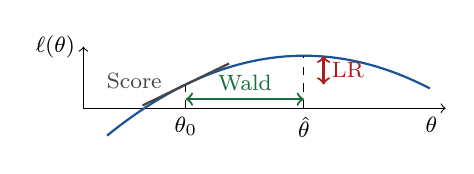
\begin{tikzpicture}[x=1.0cm,y=0.58cm,font=\fontsize{8}{9}\selectfont]
\draw[->] (0,0)--(4.6,0) node[below left]{$\theta$};
\draw[->] (0,0)--(0,1.35) node[left]{$\ell(\theta)$};
\draw[thick,cWissen,domain=0.3:4.4,samples=50] plot (\x,{1.15-0.28*(\x-2.8)*(\x-2.8)});
\draw[dashed] (2.8,0)--(2.8,1.15); \node[below] at (2.8,0){$\hat\theta$};
\draw[dashed] (1.3,0)--(1.3,0.52); \node[below] at (1.3,0){$\theta_0$};
\draw[cFalle,thick,<->] (3.05,0.52)--(3.05,1.15); \node[cFalle,right] at (3.05,0.83){LR};
\draw[cRechnen,thick,<->] (1.3,0.2)--(2.8,0.2); \node[cRechnen,above] at (2.05,0.2){Wald};
\draw[cCode,thick] (0.75,0.06)--(1.85,0.98); \node[cCode,left] at (1.1,0.6){Score};
\end{tikzpicture}
\end{center}
\begin{itemize}
\item \textbf{Wald:} $W=(\hat\theta-\theta_0)^2\,I(\hat\theta)$: horizontaler Abstand, braucht den MLE. $W=Z^2$ mit $Z=\frac{\hat\theta-\theta_0}{se(\hat\theta)}\asim N(0,1)$, daher $W\asim\chi^2_1$. Zweiseitig ist $|Z|>z_{1-\alpha/2}$ dasselbe wie $W>\chi^2_{1,1-\alpha}$. Einseitig geht nur mit $Z$ (Quadrat verliert das Vorzeichen). Wald-KI = $\hat\theta\pm z_{1-\alpha/2}\cdot se$.
\item \textbf{Score:} $S=\frac{s(\theta_0)^2}{I(\theta_0)}$: Steigung bei $\theta_0$, kein MLE nötig.
\item \textbf{LR:} $LR=2\big\{\ell(\hat\theta)-\ell(\theta_0)\big\}$: vertikaler Abstand.
\end{itemize}
$H_0:\theta=\theta_0$. Unter $H_0$ alle drei $\asim\chi^2_1$ (allg.\ $\chi^2_p$, $p$ = Anzahl Restriktionen), asymptotisch äquivalent; ablehnen, wenn $>\chi^2_{p,1-\alpha}$.
\end{wissen}
\begin{werkzeug}{Verteilungen: Dichte, Erwartungswert, Varianz}
{\everymath{\displaystyle}\renewcommand{\arraystretch}{1.55}\begin{tabularx}{\linewidth}{@{}>{\raggedright\arraybackslash}p{1.75cm}>{\raggedright\arraybackslash}X>{\raggedright\arraybackslash}p{2.75cm}@{}}
\toprule
 & Dichte / Wkt.-Funktion & $\E(X)$ ; $\V(X)$ \\
\midrule
$Bern(\pi)$ & $\pi^x(1-\pi)^{1-x}$ & $\pi$ ; $\pi(1-\pi)$ \\
$Bin(n,\pi)$ & $\binom nx\pi^x(1-\pi)^{n-x}$ & $n\pi$ ; $n\pi(1-\pi)$ \\
$Pois(\lambda)$ & $\frac{\lambda^x}{x!}e^{-\lambda}$ & $\lambda$ ; $\lambda$ \\
Geom$(p)$ & $p(1-p)^{x-1}$, $x\ge 1$ & $\frac1p$ ; $\frac{1-p}{p^2}$ \\
$Exp(\lambda)$ & $\lambda e^{-\lambda x}$; \ $F=1-e^{-\lambda x}$ & $\frac1\lambda$ ; $\frac{1}{\lambda^2}$ \\
Gamma$(\alpha,\beta)$ & $\frac{\beta^\alpha}{\Gamma(\alpha)}x^{\alpha-1}e^{-\beta x}$, $x>0$ & $\frac\alpha\beta$ ; $\frac{\alpha}{\beta^2}$ \\
Beta$(\alpha,\beta)$ & $\frac{\Gamma(\alpha+\beta)}{\Gamma(\alpha)\Gamma(\beta)}x^{\alpha-1}(1-x)^{\beta-1}$ & $\frac{\alpha}{\alpha+\beta}$ ; $\frac{\alpha\beta}{(\alpha+\beta)^2(\alpha+\beta+1)}$ \\
$N(\mu,\sigma^2)$ & $\frac{1}{\sqrt{2\pi\sigma^2}}\exp\!\big(-\frac{(x-\mu)^2}{2\sigma^2}\big)$ & $\mu$ ; $\sigma^2$ \\
$U[a,b]$ & $\frac{1}{b-a}$ & $\frac{a+b}{2}$ ; $\frac{(b-a)^2}{12}$ \\
Pareto$(m,\alpha)$ & $\frac{\alpha m^\alpha}{x^{\alpha+1}}$, $x\ge m$ & $\frac{\alpha m}{\alpha-1}$ ($\alpha>1$) \\
$\chi^2_n$ & $\sum_{i=1}^n Z_i^2$, $Z_i\iid N(0,1)$ & $n$ ; $2n$ \\
$t_n$ & $Z/\sqrt{\chi^2_n/n}$ & $0$ ; $\frac{n}{n-2}$ \\
\bottomrule
\end{tabularx}}
\end{werkzeug}


\begin{rechnen}{MLE-Katalog (zum Kontrollieren der eigenen Rechnung)}
\begin{tabularx}{\linewidth}{@{}>{\raggedright\arraybackslash}X>{\raggedright\arraybackslash}p{2.35cm}>{\raggedright\arraybackslash}p{1.7cm}@{}}
\toprule
Modell & $\hat\theta_{ML}$ & $I_n(\theta)$ \\
\midrule
$Pois(\lambda)$ & $\bar x$ & $\frac n\lambda$ \\
$Bern(\pi)$ & $\bar x$ & $\frac{n}{\pi(1-\pi)}$ \\
$Exp(\lambda)$: $\lambda e^{-\lambda x}$ & $\frac{1}{\bar x}$ & $\frac{n}{\lambda^2}$ \\
$Exp$ mit Mittel $\theta$: $\frac1\theta e^{-x/\theta}$ & $\bar x$ & $\frac{n}{\theta^2}$ \\
$N(\mu,\sigma^2)$, $\sigma^2$ bekannt & $\bar x$ & $\frac{n}{\sigma^2}$ \\
$N(\mu,\sigma^2)$, $\mu$ bekannt & $\frac1n\sum(x_i-\mu)^2$ & $\frac{n}{2\sigma^4}$ \\
Geom $p(1-p)^{x-1}$ & $\frac{1}{\bar x}$ & $\frac{n}{p^2(1-p)}$ \\
$\theta x^{\theta-1}$, $0<x<1$ & $-\frac{n}{\sum\log x_i}$ & $\frac{n}{\theta^2}$ \\
Pareto, $m$ bekannt & $\frac{n}{\sum\log(x_i/m)}$ & $\frac{n}{\alpha^2}$ \\
$U[0,\theta]$ & $x_{\max}$ & nicht regulär \\
\bottomrule
\end{tabularx}
\end{rechnen}
\end{multicols*}
\newpage
% ===================== SEITE 2: A2 Tests =====================
\begin{multicols*}{3}
\sect{A2 $\cdot$ Tests}
\begin{wissen}{Test erkennen + Annahmen nennen}
\begin{itemize}
\item \textbf{1 Mittelwert:} $\sigma^2$ bekannt \ra{} Gauß-Test; unbekannt \ra{} $t$-Test, $df=n-1$. Annahme: $X_i\iid N(\mu,\sigma^2)$ (oder $n$ groß, ZGWS).
\item \textbf{2 unabhängige Stichproben:} gleiche unbekannte Varianzen \ra{} gepoolter $t$-Test, $df=n+m-2$; ungleich \ra{} Welch. Annahmen: $X_i\iid N(\mu_X,\sigma^2)$, $Y_j\iid N(\mu_Y,\sigma^2)$, alle unabhängig.
\item \textbf{Gepaart} (dieselbe Einheit zweimal gemessen, z.B.\ vorher/nachher): $D_i=X_i-Y_i$, Einstichproben-$t$-Test mit $S_D$, $df=n-1$. Zweistichprobentest wäre falsch: ignoriert die Abhängigkeit; bei positiver Korrelation ist sein $SE$ zu groß \ra{} weniger Power.
\end{itemize}
\end{wissen}
\begin{rechnen}{Teststatistiken (Formel hinschreiben gibt Punkte)}
{\renewcommand{\arraystretch}{1.5}\begin{tabularx}{\linewidth}{@{}>{\raggedright\arraybackslash}p{1.25cm}>{\raggedright\arraybackslash}X>{\raggedright\arraybackslash}p{1.35cm}@{}}
\toprule
Test & Statistik & unter $H_0$ \\
\midrule
Gauß & $Z=\dfrac{\bar X-\mu_0}{\sigma/\sqrt n}$ & $N(0,1)$ \\
$t$ & $T=\dfrac{\bar X-\mu_0}{S/\sqrt n}$ & $t_{n-1}$ \\
gepaart & $T=\dfrac{\bar D-\delta_0}{S_D/\sqrt n}$ & $t_{n-1}$ \\
gepoolt & $T=\dfrac{\bar X-\bar Y-\delta_0}{S_p\sqrt{\frac1n+\frac1m}}$, \ $S_p^2=\frac{(n-1)S_X^2+(m-1)S_Y^2}{n+m-2}$ & $t_{n+m-2}$ \\
Welch & $T=\dfrac{\bar X-\bar Y-\delta_0}{\sqrt{S_X^2/n+S_Y^2/m}}$ & $\approx t_{df}$ \\
\bottomrule
\end{tabularx}}
Allgemein: $T=\dfrac{\text{Schätzer}-\text{Wert unter }H_0}{SE}$. Großes $df$: $t_{df}\approx N(0,1)$, also $z$-Quantile benutzen (begründen!).
\end{rechnen}
\begin{wissen}{Hypothesen aufstellen}
\textbf{Ein- oder zweiseitig:} steht fast immer direkt da: in der Aufgabe (,,einseitiger Test'') oder im R-Output (\texttt{not equal to} = zweiseitig, \texttt{greater}/\texttt{less} = einseitig). Sonst aus der Fragestellung: gefragt ist nur, \emph{ob ein Unterschied} besteht \ra{} zweiseitig; gefragt ist eine \emph{Richtung} (wirkt, senkt, erhöht, besser, mehr als) \ra{} einseitig.
\textbf{Aufstellen:} Was gezeigt werden soll, gehört in $H_1$; Gleichheit steht immer in $H_0$. Über Parameter ($\mu$) formulieren, nie über $\bar x$. Z.B.\ ,,Behandlung senkt das Gewicht'': $H_0:\mu_{vor}-\mu_{nach}\le 0$ vs.\ $H_1:\mu_{vor}-\mu_{nach}>0$.
\end{wissen}
\begin{rechnen}{Entscheidung + p-Wert interpretieren}
\textbf{3 äquivalente Wege:} (1) $|t_{obs}|>$ kritischer Wert; \ (2) $p\le\alpha$; \ (3) Wert unter $H_0$ liegt nicht im $(1-\alpha)$-KI (zweiseitig).
\textbf{Ablehnbereich:} $H_1:\theta\neq\theta_0$: $|T|>q_{1-\alpha/2}$. \ $H_1:\theta>\theta_0$: $T>q_{1-\alpha}$. \ $H_1:\theta<\theta_0$: $T<-q_{1-\alpha}$.
\textbf{p-Wert} $=P_{H_0}(T$ mindestens so extrem wie $t_{obs})$: Wahrscheinlichkeit, unter $H_0$ ein mindestens so extremes Ergebnis wie das beobachtete zu erhalten. Normal-Näherung: zweiseitig $p=2\big(1-\Phi(|t_{obs}|)\big)$, einseitig ($>$) $p=1-\Phi(t_{obs})$.
\end{rechnen}

\begin{falle}{Interpretation}
$p$-Wert $\neq P(H_0\text{ wahr})$. \ Nicht verworfen heißt nicht ,,$H_0$ bewiesen'' (evtl.\ zu kleines $n$). \ Signifikant heißt nicht relevant (großes $n$). \ Frequentistisches 95\,\%-KI: das Verfahren überdeckt $\theta$ in 95\,\% der Wiederholungen (nicht: ,,$\theta$ liegt mit 95\,\% darin''). \ Zweiseitig $\neq$ Zweistichproben.
\end{falle}
\begin{rechnen}{Güte berechnen: Rezept}
$G(\theta)=P_\theta(H_0\text{ ablehnen})$.
\begin{enumerate}[leftmargin=10pt]
\item \textbf{$SE$ bestimmen:} $\frac{\sigma}{\sqrt n}$, $\frac{S}{\sqrt n}$, $\frac{S_D}{\sqrt n}$ (gepaart), $S_p\sqrt{\frac1n+\frac1m}$. $t$-Test mit großem $n$: Normalverteilung als Näherung.
\item \textbf{Ablehnbereich auf die Schätzer-Skala umrechnen:} bei $H_1:\theta>\theta_0$ wird abgelehnt, wenn
$$\hat\theta>c=\theta_0+z_{1-\alpha}\cdot SE.$$
\item \textbf{Unter dem wahren $\theta_1$} ist $\hat\theta\sim N(\theta_1,SE^2)$: mit $\theta_1$ standardisieren, \textbf{nicht} mit $\theta_0$.
\item \textbf{Ausrechnen:}
$$G(\theta_1)=P(\hat\theta>c\mid\theta_1)=1-\Phi\Big(\frac{c-\theta_1}{SE}\Big)=\Phi\Big(\frac{\theta_1-\theta_0}{SE}-z_{1-\alpha}\Big)$$
\item \textbf{Satz:} ,,Ist der wahre Unterschied $\theta_1$, verwirft der Test $H_0$ mit Wkt.\ $G(\theta_1)$; mit $1-G(\theta_1)$ Fehler 2.\ Art.''
\end{enumerate}
Mit $\Delta=\theta_1-\theta_0$:
\begin{itemize}
\item $H_1:\theta<\theta_0$: \ $G=\Phi\big(-z_{1-\alpha}-\frac{\Delta}{SE}\big)$
\item zweiseitig: \ $G=1-\Phi\big(z_{1-\alpha/2}-\frac{\Delta}{SE}\big)+\Phi\big(-z_{1-\alpha/2}-\frac{\Delta}{SE}\big)$; der zweite Summand ist meist $\approx 0$.
\end{itemize}
\textbf{Güte steigt}, wenn $|\Delta|$, $n$ oder $\alpha$ größer bzw.\ $\sigma$ kleiner wird.
\end{rechnen}
\begin{wissen}{Güte skizzieren: Achsen, $\theta_0$, $\alpha$ und $1$ beschriften}
\begin{center}
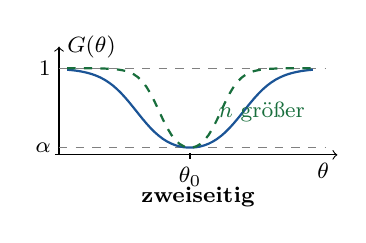
\begin{tikzpicture}[x=0.52cm,y=1.1cm,font=\fontsize{8}{9}\selectfont]
\draw[->] (-3.3,0)--(3.6,0) node[below left]{$\theta$};
\draw[->] (-3.2,0)--(-3.2,1.25) node[right]{$G(\theta)$};
\draw[dashed,gray] (-3.2,0.083)--(3.3,0.083); \node[left] at (-3.2,0.083){$\alpha$};
\draw[dashed,gray] (-3.2,1)--(3.3,1); \node[left] at (-3.2,1){$1$};
\draw[thick,cWissen,domain=-3:3,samples=60] plot (\x,{1-0.5*(1+tanh(0.8*(1.96-1.5*\x)))+0.5*(1+tanh(0.8*(-1.96-1.5*\x)))});
\draw[thick,cRechnen,dashed,domain=-3:3,samples=60] plot (\x,{1-0.5*(1+tanh(0.8*(1.96-2.6*\x)))+0.5*(1+tanh(0.8*(-1.96-2.6*\x)))});
\draw (0,0.02)--(0,-0.05) node[below]{$\theta_0$};
\node[cRechnen] at (1.75,0.5){$n$ größer};
\node[below] at (0.2,-0.28){\textbf{zweiseitig}};
\end{tikzpicture}\hspace{4pt}
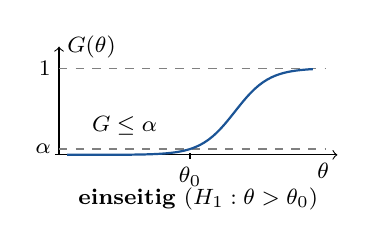
\begin{tikzpicture}[x=0.52cm,y=1.1cm,font=\fontsize{8}{9}\selectfont]
\draw[->] (-3.3,0)--(3.6,0) node[below left]{$\theta$};
\draw[->] (-3.2,0)--(-3.2,1.25) node[right]{$G(\theta)$};
\draw[dashed,gray] (-3.2,0.067)--(3.3,0.067); \node[left] at (-3.2,0.067){$\alpha$};
\draw[dashed,gray] (-3.2,1)--(3.3,1); \node[left] at (-3.2,1){$1$};
\draw[thick,cWissen,domain=-3:3,samples=60] plot (\x,{0.5*(1+tanh(0.8*(1.5*\x-1.645)))});
\draw (0,0.02)--(0,-0.05) node[below]{$\theta_0$};
\node at (-1.6,0.33){$G\le\alpha$};
\node[below] at (0.2,-0.28){\textbf{einseitig} ($H_1:\theta>\theta_0$)};
\end{tikzpicture}
\end{center}
$x$-Achse: wahrer Parameter (z.B.\ $\mu_X-\mu_Y$), $y$-Achse: Ablehnwahrscheinlichkeit. \textbf{Zweiseitig:} U-förmig um $\theta_0$, Minimum $G(\theta_0)=\alpha$, $\to 1$ nach außen. \textbf{Einseitig:} monoton steigend, $G(\theta_0)=\alpha$.
\end{wissen}
\begin{werkzeug}{R-Output lesen, fehlende Werte berechnen}
\begin{itemize}
\item Kopfzeile = Test: \texttt{One Sample t-test} ($df=n-1$), \texttt{Two Sample t-test} (gepoolt, $df=n+m-2$), \texttt{Welch Two Sample t-test}, \texttt{Paired t-test} ($df=n-1$).
\item \texttt{alternative hypothesis: ... not equal to 100} = $H_1$ zweiseitig, $\mu_0=100$ (\texttt{less}/\texttt{greater}: einseitig).
\item \textbf{Fehlendes $t$:} $t=\frac{\bar x-\mu_0}{s/\sqrt n}$ bzw.\ $\frac{\bar x-\bar y}{SE}$. \textbf{Fehlendes $df$:} aus $n$ (s.o.).
\item Schätzer = Mitte des KI. \ $SE=\frac{\text{Schätzer}-\text{Wert unter }H_0}{t}$.
\end{itemize}
\end{werkzeug}
\begin{wissen}{Fehlerarten, Sensitivität, Spezifität ($\hat y$ = Test, $y$ = Wahrheit)}
{\renewcommand{\arraystretch}{1.25}\begin{tabularx}{\linewidth}{@{}>{\raggedright\arraybackslash}p{1.95cm}|>{\raggedright\arraybackslash}X|>{\raggedright\arraybackslash}X@{}}
 & $y=1$ (krank, $H_1$ wahr) & $y=0$ (gesund, $H_0$ wahr) \\
\hline
$\hat y=1$ (Test $+$, $H_0$ verworfen) & \textbf{TP} richtig positiv & \textbf{FP} falsch positiv = \textbf{Fehler 1.\ Art} \\
\hline
$\hat y=0$ (Test $-$, $H_0$ behalten) & \textbf{FN} falsch negativ = \textbf{Fehler 2.\ Art} & \textbf{TN} richtig negativ \\
\end{tabularx}}
\textbf{Spaltenweise} (gegeben Wahrheit, unabhängig von Prävalenz):
\begin{itemize}
\item \textbf{Sensitivität} = Recall = Trefferquote = True Positive Rate (TPR) = Power $=\frac{TP}{TP+FN}=P(+\mid\text{krank})$
\item \textbf{Spezifität} = True Negative Rate (TNR) $=\frac{TN}{TN+FP}=P(-\mid\text{gesund})$
\item False Positive Rate $=1-$Spez ($\widehat{=}\,\alpha$), False Negative Rate $=1-$Sens ($\widehat{=}\,\beta$)
\end{itemize}
\textbf{Zeilenweise} (gegeben Testergebnis, \textbf{abhängig von Prävalenz $p$}):
\begin{itemize}
\item \textbf{PPV} = Precision = positiver prädiktiver Wert $=\frac{TP}{TP+FP}=P(\text{krank}\mid +)=\frac{\text{Sens}\cdot p}{\text{Sens}\cdot p+(1-\text{Spez})(1-p)}$
\item \textbf{NPV} = negativer prädiktiver Wert $=\frac{TN}{TN+FN}=P(\text{gesund}\mid -)$, analog über Bayes
\end{itemize}
Accuracy $=\frac{TP+TN}{N}$. \textbf{Im Kontext:} Fehler 1.\ Art = $H_0$ stimmt, man entscheidet für $H_1$ (Wkt.\ $\le\alpha$). Fehler 2.\ Art = $H_1$ stimmt, man behält $H_0$ (Wkt.\ $\beta=1-G(\theta)$). Festes $n$: $\alpha\downarrow$ \ra{} $\beta\uparrow$.
\end{wissen}


\begin{rechnen}{KI auf anderes Niveau umrechnen, kritische Werte}
\begin{enumerate}[leftmargin=10pt]
\item Schätzer $=\frac{u+o}{2}$ (Mitte des gegebenen KI $[u,o]$).
\item $SE$ beschaffen, einer der Wege: \ $SE=\frac{o-u}{2\,q_{1-\alpha/2}}$ (mit dem Quantil des \emph{alten} Niveaus); \ $SE=\frac{\text{Schätzer}}{t}$ (aus R-Output, $H_0$-Wert 0); \ $SE=\hat\sigma_p\sqrt{\frac1n+\frac1m}$.
\item Neues KI: Schätzer $\pm\,q_{1-\alpha'/2}\cdot SE$.
\end{enumerate}
Kleineres Niveau \ra{} kleineres Quantil \ra{} schmaleres KI. \textbf{Falle:} gegebenes $\hat\sigma$ (gepoolte SD der Einzelwerte) ist \emph{nicht} der $SE$: erst mit $\sqrt{\frac1n+\frac1m}$ multiplizieren.
\textbf{Kritische Werte bei anderem $\alpha$:} zweiseitig $\pm q_{1-\alpha/2}$, einseitig $q_{1-\alpha}$; $|t_{obs}|$ damit vergleichen. \textbf{$t$ durch $N(0,1)$ ersetzen:} $t_{df}\to N(0,1)$ für $df\to\infty$, ab etwa $df\ge 30$ praktisch gleich; bei kleinem $df$ wäre $z$ zu liberal.
\end{rechnen}
\begin{wissen}{Multiples Testen}
\textbf{Problem:} Bei $m$ Tests je zum Niveau $\alpha$ steigt die Wkt.\ für \emph{mindestens einen} Fehler 1.\ Art: $FWER=1-(1-\alpha)^m$ (unabhängige Tests) $\le m\alpha$.
\textbf{Bonferroni:} jeden Test zum Niveau $\frac{\alpha}{m}$ (gleichwertig: $m\cdot p_j\le\alpha$) \ra{} $FWER\le m\cdot\frac{\alpha}{m}=\alpha$, bei jeder Abhängigkeit. Konservativ, weniger Power. Antwort: $p$ mit $\frac{\alpha}{m}$ vergleichen.
\end{wissen}




\begin{rechnen}{W/F-Klassiker: Tests}
\begin{wftab}
$p$-Wert $=P(H_0$ wahr$)$ & \F & $p=P_{H_0}$(Statistik mindestens so extrem wie beobachtet). \\
Spezifität 0.95 \ra{} bei negativem Test mit 95\,\% gesund & \F & Spezifität $=P(-\mid$gesund$)$. Gefragt ist $P($gesund$\mid -)$ = NPV; hängt über Bayes von der Prävalenz ab. \\
Nicht verworfen \ra{} $H_0$ ist wahr & \F & nur keine ausreichende Evidenz dagegen (evtl.\ $n$ zu klein). \\
Signifikant \ra{} praktisch relevant & \F & bei großem $n$ werden auch winzige Effekte signifikant. \\
Power $=1-\alpha$ & \F & Power $=1-\beta(\theta)$, hängt vom wahren $\theta$ ab. \\
\end{wftab}
\end{rechnen}
\end{multicols*}
\newpage
% ===================== SEITE 3: A3 Bayes =====================
\begin{multicols*}{3}
\sect{A3 $\cdot$ Bayes}
\begin{wissen}{Prinzip}
Daten $y_i\mid\theta\sim f(y\mid\theta)$, Prior $p(\theta)$: $\theta$ ist eine Zufallsvariable, die unsere Unsicherheit über $\theta$ beschreibt.
$$p(\theta\mid y)=\frac{\prod_i f(y_i\mid\theta)\cdot p(\theta)}{f(y)}\ \propto\ \underbrace{L(\theta)}_{\text{Likelihood}}\cdot\underbrace{p(\theta)}_{\text{Prior}}$$
$f(y)=\int L(\theta)p(\theta)\,d\theta$ hängt nicht von $\theta$ ab (Normierungskonstante) und wird fast nie gebraucht.
\textbf{Konjugiert:} Die Posterior liegt in derselben Verteilungsfamilie wie der Prior.
\end{wissen}
\begin{rechnen}{Rezept: Posterior bis auf Konstante herleiten}
\begin{enumerate}[leftmargin=10pt]
\item \textbf{Likelihood der ganzen Stichprobe} ausschreiben und zusammenfassen: $\prod_i\lambda^{y_i}=\lambda^{\sum y_i}$, \ $\prod_ie^{-\lambda}=e^{-n\lambda}$, \ $\prod_i\sqrt\tau=\tau^{n/2}$, \ $\prod_i\ind\{x_i\le\theta\}=\ind\{\theta\ge x_{\max}\}$ (Indikator: $\ind\{A\}=1$, wenn $A$ gilt, sonst $0$; das Produkt ist nur $1$, wenn \emph{alle} $x_i\le\theta$, also $\theta\ge$ größtes $x_i$).
\item \textbf{Prior-Kern} dazuschreiben (nur die Teile mit $\theta$).
\item \textbf{Alles ohne $\theta$ streichen}, mit Begründung ,,Normierungskonstante, hängt nicht von $\theta$ ab'': z.B.\ $\frac{1}{y_i!}$, $\frac{\beta^\alpha}{\Gamma(\alpha)}$, $\frac{1}{\sqrt{2\pi}}$.
\item \textbf{Gleiche Basen zusammenfassen:} Exponenten addieren, $\theta^a\cdot\theta^b=\theta^{a+b}$, $e^{-a\theta}\cdot e^{-b\theta}=e^{-(a+b)\theta}$. Indikatoren kombinieren: $\ind\{\theta\ge a\}\cdot\ind\{\theta\ge b\}=\ind\{\theta\ge\max(a,b)\}$.
\item \textbf{Kern erkennen} (Tabelle unten), neue Parameter $\alpha^*,\beta^*$ ablesen. Satz: ,,Die Posterior hat den Kern einer Gamma-Verteilung, also $\theta\mid y\sim$ Gamma$(\alpha^*,\beta^*)$. Gleiche Familie wie der Prior \ra{} konjugiert.''
\end{enumerate}
\end{rechnen}
\begin{werkzeug}{Kerne (als Funktion von $\theta$) und Kennzahlen}
{\renewcommand{\arraystretch}{1.3}\begin{tabularx}{\linewidth}{@{}>{\raggedright\arraybackslash}p{1.95cm}>{\raggedright\arraybackslash}p{2.55cm}>{\raggedright\arraybackslash}X@{}}
\toprule
Verteilung & Kern & Erwartungswert; Modus; Varianz \\
\midrule
Beta$(\alpha,\beta)$ & $\theta^{\alpha-1}(1-\theta)^{\beta-1}$, $\theta\in(0,1)$ & $\frac{\alpha}{\alpha+\beta}$; \ $\frac{\alpha-1}{\alpha+\beta-2}$ ($\alpha,\beta>1$); \ $\frac{\alpha\beta}{(\alpha+\beta)^2(\alpha+\beta+1)}$ \\
Gamma$(\alpha,\beta)$ & $\theta^{\alpha-1}e^{-\beta\theta}$, $\theta>0$ & $\frac\alpha\beta$; \ $\frac{\alpha-1}{\beta}$ ($\alpha\ge 1$); \ $\frac{\alpha}{\beta^2}$ \\
IG$(\alpha,\beta)$ & $\theta^{-\alpha-1}e^{-\beta/\theta}$, $\theta>0$ & $\frac{\beta}{\alpha-1}$; \ $\frac{\beta}{\alpha+1}$; \ $\frac{\beta^2}{(\alpha-1)^2(\alpha-2)}$ \\
$N(\mu,\sigma^2)$ & $\exp\!\big(-\frac{A}{2}\theta^2+B\theta\big)$ & $\mu=\frac BA$ (= Modus = Median); \ $\sigma^2=\frac1A$ \\
Pareto$(m,\alpha)$ & $\theta^{-(\alpha+1)}\,\ind\{\theta\ge m\}$ & $\frac{\alpha m}{\alpha-1}$ ($\alpha>1$); \ $m$; \ $F(\theta)=1-\big(\frac m\theta\big)^\alpha$ \\
\bottomrule
\end{tabularx}}
Gamma in Shape-Rate-Form. IG = Inverse Gamma: $\tau\sim$ Gamma$(\alpha,\beta)$ $\Leftrightarrow$ $\frac1\tau\sim$ IG$(\alpha,\beta)$.
\textbf{Normal-Kern erkennen:} Exponent der Posterior nach Potenzen von $\theta$ ordnen: $-\frac A2\theta^2+B\theta+$ (Rest ohne $\theta$). $A$ = $-2\times$ Faktor vor $\theta^2$, $B$ = Faktor vor $\theta$. Dann $\theta\mid y\sim N\big(\frac BA,\ \frac1A\big)$. Beispiel Normal-Normal: $A=\frac{n}{\sigma^2}+\frac{1}{\tau^2}$, $B=\frac{\sum y_i}{\sigma^2}+\frac{\delta}{\tau^2}$.
\end{werkzeug}

\begin{rechnen}{Konjugierte Paare}
{\renewcommand{\arraystretch}{1.35}\begin{tabularx}{\linewidth}{@{}>{\raggedright\arraybackslash}p{2.25cm}>{\raggedright\arraybackslash}p{1.95cm}>{\raggedright\arraybackslash}X@{}}
\toprule
Daten & Prior & Posterior \\
\midrule
$Bin(n,\pi)$: $y$ Erfolge & Beta$(\alpha,\beta)$ & Beta$(\alpha+y,\ \beta+n-y)$ \\
$Bern(\pi)$, $n$ Beob. & Beta$(\alpha,\beta)$ & Beta$(\alpha+\sum y_i,\ \beta+n-\sum y_i)$ \\
Geom $\pi(1-\pi)^{x-1}$ & Beta$(\alpha,\beta)$ & Beta$(\alpha+n,\ \beta+\sum x_i-n)$ \\
$Pois(\lambda)$ & Gamma$(\alpha,\beta)$ & Gamma$(\alpha+\sum y_i,\ \beta+n)$ \\
$Exp(\lambda)$ & Gamma$(\alpha,\beta)$ & Gamma$(\alpha+n,\ \beta+\sum x_i)$ \\
$N(\mu_0,\frac1\tau)$, Präzision $\tau$ & Gamma$(\alpha,\beta)$ & Gamma$\big(\alpha+\frac n2,\ \beta+\frac12\sum(y_i-\mu_0)^2\big)$ \\
$N(\mu_0,\sigma^2)$, Varianz $\sigma^2$ & IG$(\alpha,\beta)$ & IG$\big(\alpha+\frac n2,\ \beta+\frac12\sum(y_i-\mu_0)^2\big)$ \\
$N(\mu,\sigma^2)$, $\sigma^2$ bekannt & $N(\delta,\tau^2)$ & $N(\mu^*,V^*)$: $\frac{1}{V^*}=\frac{n}{\sigma^2}+\frac{1}{\tau^2}$, \ $\mu^*=V^*\big(\frac{\sum y_i}{\sigma^2}+\frac{\delta}{\tau^2}\big)$ \\
$U(0,\theta)$ & Pareto$(m,\alpha)$ & Pareto$\big(\max(m,x_{\max}),\ \alpha+n\big)$ \\
\bottomrule
\end{tabularx}}
\textbf{Posterior-Erwartungswert = gewichtetes Mittel aus Daten und Prior:} Beta-Bin: $\frac{\alpha+y}{\alpha+\beta+n}=w\frac yn+(1-w)\frac{\alpha}{\alpha+\beta}$, $w=\frac{n}{\alpha+\beta+n}$. Gamma-Pois: $\frac{\alpha+\sum y_i}{\beta+n}=w\bar y+(1-w)\frac\alpha\beta$, $w=\frac{n}{\beta+n}$. Normal: Präzisionen addieren sich. Für $n\to\infty$ geht $w\to 1$: der Prior verliert an Einfluss.
\end{rechnen}
\begin{wissen}{Mit der Posterior arbeiten}
\textbf{Punktschätzer:} Posterior-Erwartungswert, Posterior-Median (bei schiefer Posterior), MAP = Modus $=\arg\max_\theta L(\theta)p(\theta)$ (ohne Normierung). \textbf{Unsicherheit:} Posterior-Standardabweichung $=\sqrt{\V(\theta\mid y)}$ oder Kredibilitätsintervall.
\textbf{Kredibilitätsintervall} $[t_l,t_r]$ mit $P(t_l\le\theta\le t_r\mid y)=1-\alpha$:
\begin{itemize}
\item \textbf{Equal-tailed:} $[q_{\alpha/2},\ q_{1-\alpha/2}]$ der Posterior (links und rechts je $\frac\alpha2$).
\item \textbf{HDI} (highest posterior density): kürzestes Intervall; jeder Punkt innen hat höhere Dichte als jeder außen. Symmetrisch und eingipflig \ra{} HDI = equal-tailed. Dichte fällt ab dem linken Rand $\theta_{\min}$ (z.B.\ Pareto) \ra{} HDI $=[\theta_{\min},\ q_{1-\alpha}]$.
\item \textbf{Transformation} $g$ monoton (z.B.\ $\sigma^2=\frac1\tau$): Quantile bzw.\ equal-tailed-Grenzen einfach transformieren; ist $g$ \textbf{fallend}, Grenzen tauschen: $\big[\frac{1}{q_{1-\alpha/2}},\ \frac{1}{q_{\alpha/2}}\big]$. Gilt nicht für HDI und nicht für den Erwartungswert (Jensen).
\item Aussage ,,$\theta$ liegt mit Wahrscheinlichkeit $1-\alpha$ im Intervall'' ist hier korrekt (beim frequentistischen KI nicht).
\end{itemize}
\textbf{Entscheidungsregel} über $P(\theta\in A\mid y)$: Ereignis auf $\theta$ umschreiben (bei fallendem $g$ Ungleichung drehen: $\sigma^2>c\Leftrightarrow\tau<\frac1c$), dann mit den gegebenen Posterior-Quantilen einordnen: liegt $\frac1c$ unter $q_{0.005}$, ist $P(\tau<\frac1c\mid y)<0.005$.
\textbf{Posterior-prädiktiv:} $f(y_{neu}\mid y)=\int f(y_{neu}\mid\theta)p(\theta\mid y)\,d\theta$; Beta-Bernoulli: $P(Y_{neu}=1\mid y)=\E(\pi\mid y)$.
\end{wissen}

\begin{falle}{Bayes-Fallen}
\begin{itemize}
\item $\E(\sigma^2\mid y)=\E\big(\frac1\tau\mid y\big)=\frac{\beta^*}{\alpha^*-1}\neq\frac{1}{\E(\tau\mid y)}=\frac{\beta^*}{\alpha^*}$.
\item Gamma in Shape-Rate ($\E(\tau)=\frac\alpha\beta$) vs.\ Shape-Scale ($\E(\tau)=\alpha\cdot$Scale): Parametrisierung der Aufgabe prüfen.
\item Pareto-Posterior: neues $m^*=\max(m,x_{\max})$, nicht $m+x_{\max}$. Dichte fällt ab $m^*$ \ra{} MAP $=m^*$, HDI beginnt bei $m^*$.
\item Normierungskonstante nur nötig, wenn Wahrscheinlichkeiten ohne gegebene Quantile verlangt sind.
\end{itemize}
\end{falle}
\begin{wissen}{Bayes-Begriffe und -Verfahren (Glossar)}
\begin{itemize}
\item \textbf{Flacher Prior} $p(\theta)\propto 1$: Posterior $\propto$ Likelihood, MAP = MLE. Auf $\mathbb R$ \textbf{improper} ($\int p=\infty$), Posterior meist trotzdem proper. Nicht invariant: flach in $\pi$ ist nicht flach in $\log\frac{\pi}{1-\pi}$.
\item \textbf{Informativer Prior:} kleine Prior-Varianz, starkes Vorwissen. \textbf{Konjugierter Prior:} Posterior in geschlossener Form, leicht zu aktualisieren; bildet echtes Vorwissen evtl.\ schlecht ab.
\item \textbf{Bernstein-von-Mises:} für $n\to\infty$ (regulär, endlich viele Parameter) gilt $\theta\mid y\asim N\big(\hat\theta_{ML},I^{-1}(\hat\theta)\big)$ \ra{} Bayes und ML liefern praktisch dasselbe, der Prior wird unwichtig.
\item \textbf{Empirical Bayes:} Hyperparameter des Priors werden aus den Daten geschätzt (ML auf der Randverteilung $f(y)$). Daten doppelt genutzt \ra{} nicht voll bayesianisch.
\item \textbf{Hierarchisches Modell:} $y_{ij}\mid\theta_j$, $\theta_j\mid\mu,\tau^2$, Hyperprior auf $(\mu,\tau^2)$. Gruppenschätzer schrumpfen zum Gesamtmittel: $\hat\theta_j=\lambda_j\bar y_j+(1-\lambda_j)\mu$, $\lambda_j=\frac{n_j\tau^2}{n_j\tau^2+\sigma^2}$. Starkes Shrinkage bei kleinem $n_j$ (,,borrowing strength''). Kompromiss zwischen ,,jede Gruppe getrennt'' (unverzerrt, hohe Varianz) und ,,alles gepoolt'' (Bias).
\item \textbf{MCMC für die Posterior:} MH mit Ziel $L(\theta)p(\theta)$, Normierung $f(y)$ kürzt sich. Nach Burn-in: Posterior-Erwartungswert = Mittel der Ziehungen, $P(\theta\in A\mid y)$ = Anteil der Ziehungen in $A$. Gibbs, wenn die bedingten Posteriors bekannt sind.
\item \textbf{ABC} (Approximate Bayesian Computation): $\theta^*$ aus dem Prior ziehen, Daten $y^*$ damit simulieren, $\theta^*$ behalten, wenn $y^*$ nah an $y$ ist ($d(y^*,y)\le\varepsilon$). Braucht keine Likelihood-Formel, nur ein Modell zum Simulieren. $\varepsilon\to 0$: exakt, aber kaum Akzeptanz; $\varepsilon\to\infty$: Ergebnis = Prior.
\item \textbf{Variational Bayes:} Posterior durch einfache Verteilung $q$ approximieren, die $KL(q\,\|\,p(\cdot\mid y))$ minimiert (gleichwertig: ELBO maximieren). Schnell und skalierbar; Approximationsfehler unbekannt, unterschätzt oft die Unsicherheit.
\item \textbf{Bayes und Regularisierung:} MAP maximiert $\ell(\theta)+\log p(\theta)$ = penalisierte Likelihood. Normal-Prior $N(0,\tau^2)$ = Ridge, Laplace-Prior = Lasso. Hilft bei kleinem $n$ oder $p>n$.
\end{itemize}
\end{wissen}


\begin{rechnen}{W/F-Klassiker: Bayes}
\begin{wftab}
Flacher Prior \ra{} MAP = MLE & \W & Posterior $\propto$ Likelihood, also dasselbe Maximum. \\
Flacher Prior ist in jeder Parametrisierung uninformativ & \F & flach in $\theta$ ist nicht flach in $g(\theta)$ (Dichtetransformation). \\
HDI = equal-tailed-Intervall & \F & nur bei symmetrischer, eingipfliger Posterior. \\
$\E(g(\theta)\mid y)=g(\E(\theta\mid y))$ & \F & nur für lineares $g$ (Jensen). \\
ABC braucht die Likelihood & \F & nur ein Modell, aus dem man simulieren kann. \\
\end{wftab}
\end{rechnen}
\begin{wissen}{Bayes vs.\ frequentistisch}
{\renewcommand{\arraystretch}{1.15}\begin{tabularx}{\linewidth}{@{}>{\raggedright\arraybackslash}p{1.6cm}>{\raggedright\arraybackslash}X>{\raggedright\arraybackslash}X@{}}
 & frequentistisch & Bayes \\
\hline
Parameter & fest, unbekannt & Zufallsvariable \\
Intervall & Verfahren überdeckt $\theta$ in $(1-\alpha)$ der Wiederholungen & $\theta$ liegt mit Wkt.\ $1-\alpha$ darin \\
Information & nur Daten & Prior + Daten \\
kleines $n$ & Asymptotik versagt (z.B.\ $\hat\pi=0$) & funktioniert, aber priorabhängig \\
großes $n$ & MLE-Asymptotik & BvM: gleiches Ergebnis \\
\end{tabularx}}
\end{wissen}
\end{multicols*}
\newpage
% ===================== SEITE 4: A3 Simulation + A4 Graphen/Missing =====================
\begin{multicols*}{3}
\sect{A3 $\cdot$ Simulation}
\begin{wissen}{Welche Methode wofür?}
\begin{itemize}
\item $F$ invertierbar \ra{} \textbf{Inversionsmethode}.
\item Dichte $f$ bekannt, ziehbare Hülle $a\cdot f^*\ge f$ \ra{} \textbf{Rejection Sampling} (exakte, unabhängige Ziehungen).
\item Nur Erwartungswert $\E_f\big(h(Y)\big)$ gesucht, aus $f$ schwer ziehbar \ra{} \textbf{Importance Sampling}.
\item $f$ nur bis auf Konstante bekannt (Posterior $\propto L\cdot p$) \ra{} \textbf{MCMC / Metropolis-Hastings}.
\item Mehrdimensional, bedingte Verteilungen bekannt \ra{} \textbf{Gibbs}.
\item $F$ unbekannt, nur Daten \ra{} \textbf{Bootstrap} (Unsicherheit eines Schätzers).
\item Test auf gleiche Verteilung ohne Verteilungsannahme \ra{} \textbf{Permutationstest}.
\end{itemize}
\textbf{Monte Carlo:} $\E\big(h(Y)\big)\approx\frac1N\sum_{i=1}^N h(Y_i)$ (GGZ); Fehler $\approx\frac{\hat\sigma}{\sqrt N}$ (ZGWS). Ein Integral $\int g(x)dx$ als Erwartungswert umschreiben, z.B.\ $\int_0^1 g(x)dx=\E\big(g(U)\big)$, $U\sim U[0,1]$.
\end{wissen}
\begin{rechnen}{Inversionsmethode: Schritte + warum + Zahl}
\textbf{Schritte:}
\begin{enumerate}[leftmargin=10pt]
\item $u=F(y)$ nach $y$ auflösen \ra{} Quantilfunktion $F^{-1}(u)$ (oft in der Aufgabe gegeben).
\item $U\sim U[0,1]$ ziehen.
\item $Y=F^{-1}(U)$ ausgeben; das ist eine Ziehung aus $F$.
\end{enumerate}
\textbf{Warum es funktioniert:} $F$ ist monoton wachsend und $P(U\le u)=u$, also
$$P(Y\le y)=P\big(F^{-1}(U)\le y\big)=P\big(U\le F(y)\big)=F(y).$$
Grafisch: $u$ auf der $y$-Achse der Verteilungsfunktion abtragen, waagerecht bis zur Kurve, senkrecht runter auf die $x$-Achse.
\textbf{Rechnen:} gegebenes $u$ in $F^{-1}$ einsetzen. $Exp(\lambda)$: $F^{-1}(u)=-\frac1\lambda\log(1-u)$. Pareto$(m,\alpha)$: $F^{-1}(u)=\frac{m}{(1-u)^{1/\alpha}}$.
\end{rechnen}
\begin{rechnen}{Rejection Sampling}
Voraussetzung: $f(y)\le a\,f^*(y)$ für alle $y$ (Hülle liegt über $f$), aus $f^*$ kann man ziehen.
\begin{enumerate}[leftmargin=10pt]
\item $Y^*\sim f^*$ ziehen, \ $U\sim U[0,1]$ ziehen.
\item Akzeptieren, falls $U\le\frac{f(Y^*)}{a\,f^*(Y^*)}$; sonst verwerfen, zurück zu 1.
\end{enumerate}
Akzeptanzwahrscheinlichkeit $=\frac1a$; im Mittel $a$ Versuche pro Ziehung. Bestes $a=\max_y\frac{f(y)}{f^*(y)}$, also $f^*$ möglichst ähnlich zu $f$ wählen. Ergebnis: exakt aus $f$ und unabhängig.
\end{rechnen}
\begin{rechnen}{Importance Sampling}
$$\E_f\big(h(Y)\big)=\int h(y)\frac{f(y)}{f^*(y)}f^*(y)\,dy\approx\frac1N\sum_{i=1}^N h(Y_i)\,w(Y_i)$$
mit $Y_i\iid f^*$ und Gewichten $w(y)=\frac{f(y)}{f^*(y)}$.
Gezogen wird aus der Vorschlagsdichte $f^*$, nicht aus $f$; die Gewichte $w$ korrigieren das. Bedingung: $f^*>0$ überall, wo $h\cdot f\neq 0$. Unverzerrt. Gut, wenn $f^*$ dort viel Masse hat, wo $|h|f$ groß ist (z.B.\ seltene Ereignisse). Ist $f$ nur bis auf Konstante bekannt: $\hat\mu=\frac{\sum h(Y_i)w_i}{\sum w_i}$. Hat $f^*$ dünnere Ränder als $f$: riesige Gewichte, instabil.
\end{rechnen}

\begin{wissen}{Metropolis-Hastings (MCMC)}
Ziel: aus $f$ ziehen, bekannt ist nur $\tilde f=c\cdot f$ (z.B.\ Posterior $\propto L\cdot p$).
\begin{enumerate}[leftmargin=10pt]
\item Startwert $Y^{(0)}$ wählen.
\item Vorschlag $Y^*\sim g(\cdot\mid Y^{(t)})$.
\item Akzeptanzwahrscheinlichkeit ($c$ kürzt sich):
$$\alpha=\min\left\{1,\ \frac{\tilde f(Y^*)}{\tilde f(Y^{(t)})}\cdot\frac{g(Y^{(t)}\mid Y^*)}{g(Y^*\mid Y^{(t)})}\right\}$$
\item $U\sim U[0,1]$: falls $U\le\alpha$ \ra{} $Y^{(t+1)}=Y^*$ (Kette bewegt sich); sonst $Y^{(t+1)}=Y^{(t)}$ (Kette bleibt stehen, der alte Wert zählt noch einmal).
\end{enumerate}
\textbf{Random Walk:} $Y^*=Y^{(t)}+\varepsilon$, $\varepsilon\sim N(0,s^2)$. Symmetrischer Vorschlag \ra{} $g$-Quotient $=1$ \ra{} $\alpha=\min\big\{1,\frac{\tilde f(Y^*)}{\tilde f(Y^{(t)})}\big\}$.
\textbf{Einzelnen Vorschlag beurteilen:} Dichte am Vorschlag höher als am aktuellen Wert \ra{} Quotient $>1$ \ra{} $\alpha=1$ \ra{} wird sicher akzeptiert. Dichte niedriger \ra{} akzeptiert mit Wahrscheinlichkeit = Dichteverhältnis. Vorschlag außerhalb des Trägers \ra{} $\tilde f=0$ \ra{} nie akzeptiert.
\textbf{Diagnostik:}
\begin{itemize}
\item \textbf{Burn-in:} Anfang der Kette verwerfen (hängt noch vom Startwert ab, Trend im Trace-Plot).
\item \textbf{Autokorrelation:} MCMC-Ziehungen sind abhängig (Markov-Kette); je höher, desto weniger Information pro Ziehung.
\item \textbf{Thinning:} nur jeden $d$-ten Wert behalten; senkt Autokorrelation, wirft aber Information weg.
\item \textbf{Akzeptanzrate:} weder sehr hoch noch sehr niedrig. Faustregel im Skript 20--30\,\% (eindimensional optimal ca.\ 44\,\%). Eine Rate in diesem Bereich ist vernünftig.
\end{itemize}
\end{wissen}
\begin{rechnen}{Trace-Plots (,,Spuren'') und Schrittweite $s$}
\begin{center}
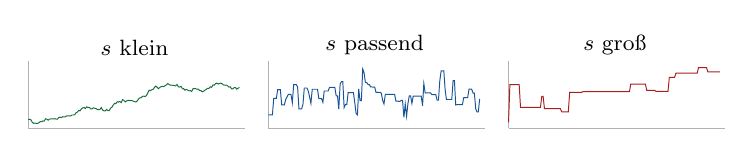
\begin{tikzpicture}[font=\fontsize{8}{9}\selectfont]
\begin{scope}
\draw[gray!60] (0,-0.4)--(2.75,-0.4); \draw[gray!60] (0,-0.4)--(0,0.45);
\traceKlein{cRechnen,line width=0.35pt}
\node[above] at (1.35,0.42){$s$ klein};
\end{scope}
\begin{scope}[xshift=3.05cm]
\draw[gray!60] (0,-0.4)--(2.75,-0.4); \draw[gray!60] (0,-0.4)--(0,0.45);
\traceGut{cWissen,line width=0.35pt}
\node[above] at (1.35,0.42){$s$ passend};
\end{scope}
\begin{scope}[xshift=6.1cm]
\draw[gray!60] (0,-0.4)--(2.75,-0.4); \draw[gray!60] (0,-0.4)--(0,0.45);
\traceGross{cFalle,line width=0.35pt}
\node[above] at (1.35,0.42){$s$ groß};
\end{scope}
\end{tikzpicture}
\end{center}
{\renewcommand{\arraystretch}{1.15}\begin{tabularx}{\linewidth}{@{}>{\raggedright\arraybackslash}p{2.15cm}>{\raggedright\arraybackslash}X>{\raggedright\arraybackslash}X@{}}
 & \textbf{$s$ klein} & \textbf{$s$ groß} \\
\hline
Trace-Plot & glatt, langsam wandernd, Trends; deckt nur kleinen Wertebereich ab & große Sprünge und lange \textbf{waagerechte Stücke} (Kette bleibt stehen) \\
Akzeptanzrate & sehr hoch: Vorschlag liegt fast am selben Punkt, Dichte fast gleich & niedrig: Vorschläge landen oft in Regionen niedriger Dichte \\
Autokorrelation & sehr hoch (Minischritte) & hoch (viele Wiederholungen desselben Werts) \\
Problem & erkundet die Posterior nur langsam & viele Vorschläge verschwendet \\
\end{tabularx}}
\textbf{Gut:} mittleres $s$, Kette springt schnell über den ganzen Bereich (,,haarige Raupe''), niedrige Autokorrelation.
\end{rechnen}

\begin{wissen}{Gibbs Sampling}
Mehrdimensional; bekannt sind die bedingten Verteilungen $f(y_j\mid y_{-j})$ (,,full conditionals''). Pro Iteration für $j=1,\dots,p$ nacheinander $Y_j$ aus $f(y_j\mid\text{aktuelle übrige Werte})$ ziehen und sofort überschreiben.
\textbf{Gibbs = MH mit Akzeptanz 1:} Vorschlag ist die full conditional; im MH-Quotienten kürzt sich alles zu $1$ \ra{} jeder Vorschlag wird angenommen.
\end{wissen}
\begin{wissen}{Bootstrap}
\textbf{Idee:} Die unbekannte Verteilung $F$ durch die empirische Verteilung $F_n$ der Daten ersetzen.
\textbf{Ablauf:} für $b=1,\dots,B$: $n$-mal \textbf{mit Zurücklegen} aus den Daten ziehen, Schätzer $\hat\theta^{*(b)}$ berechnen. Dann: $\widehat{SE}$ = Standardabweichung der $\hat\theta^{*(b)}$; Perzentil-KI $=[\hat\theta^*_{(\alpha/2)},\ \hat\theta^*_{(1-\alpha/2)}]$ (Quantile der Bootstrap-Schätzer); Bias $\approx\bar\theta^*-\hat\theta$.
\textbf{Parametrischer Bootstrap:} aus $F(\cdot;\hat\theta)$ simulieren statt aus den Daten.
\end{wissen}
\begin{falle}{Wann Bootstrap nicht funktioniert}
\begin{itemize}
\item $B\to\infty$ entfernt nur den Simulationsfehler: man erhält die Verteilung von $\hat\theta^*$ unter $F_n$, nicht unter $F$. Für die wahre Verteilung braucht man $n\to\infty$.
\item \textbf{Kleines $n$:} $F_n$ approximiert $F$ schlecht, es gibt nur wenige verschiedene Resamples.
\item \textbf{Maximum/Randschätzer} ($\hat\theta=x_{\max}$): Bootstrap-Werte sind nie größer als $x_{\max}$, obwohl $\theta\ge x_{\max}$; $x_{\max}$ wird mit großer Wahrscheinlichkeit $1-(1-\frac1n)^n$ erneut gezogen \ra{} Punktmasse, Unsicherheit unterschätzt. Grund: Schätzer ist nicht glatt, Situation nicht regulär.
\end{itemize}
\end{falle}
\begin{wissen}{Permutationstest}
$H_0$: beide Gruppen haben dieselbe Verteilung \ra{} Gruppenlabels sind vertauschbar. Daten poolen, Labels \textbf{ohne Zurücklegen} neu verteilen (alle oder viele Permutationen), jeweils Teststatistik berechnen. $p$-Wert = Anteil der permutierten Statistiken, die mindestens so extrem sind wie die beobachtete. Keine Normalverteilungsannahme nötig, nur Vertauschbarkeit unter $H_0$.
\end{wissen}

\begin{rechnen}{W/F-Klassiker: Simulation}
\begin{wftab}
Bootstrap: für $B\to\infty$ konvergiert die Bootstrap-Verteilung gegen die wahre Verteilung von $\hat\theta$ & \F & $B\to\infty$ entfernt nur den Simulationsfehler; man bleibt bei $F_n$ statt $F$. Dafür bräuchte man $n\to\infty$. \\
Bootstrap zieht ohne Zurücklegen & \F & mit Zurücklegen; ohne Zurücklegen = Permutationstest. \\
Importance Sampling zieht aus der Zielverteilung & \F & gezogen wird aus der Vorschlagsdichte $f^*$, die Gewichte $w=\frac{f}{f^*}$ korrigieren. \\
Rejection Sampling liefert exakte, unabhängige Ziehungen & \W & akzeptierte Werte sind genau $\sim f$; Akzeptanzwahrscheinlichkeit $\frac1a$. \\
MH braucht die Normierungskonstante & \F & sie kürzt sich im Quotienten $\frac{\tilde f(Y^*)}{\tilde f(Y^{(t)})}$. \\
MCMC-Ziehungen sind unabhängig & \F & Markov-Kette: jeder Wert hängt vom vorherigen ab \ra{} Autokorrelation. \\
Hohe Akzeptanzrate = gute Kette & \F & sehr hohe Rate heißt meist winzige Schritte, hohe Autokorrelation, langsame Erkundung. \\
Gibbs ist ein Spezialfall von MH mit Akzeptanz 100\,\% & \W & Vorschlag = full conditional \ra{} MH-Quotient $=1$. \\
\end{wftab}
\end{rechnen}
\end{multicols*}
\newpage
% ===================== SEITE 5: A4 =====================
\begin{multicols*}{3}
\sect{A4 $\cdot$ Graphen-Aufgabe (bedingte Unabhängigkeit)}
\begin{wissen}{Ungerichtete Graphen}
$A\indep B\mid C$ heißt: $f(y_A,y_B\mid y_C)=f(y_A\mid y_C)\,f(y_B\mid y_C)$. \textbf{Fehlende Kante = bedingt unabhängig gegeben alle übrigen Variablen.}
\textbf{Rezept ,,alle bedingten Unabhängigkeiten auflisten'':}
\begin{enumerate}[leftmargin=10pt]
\item \textbf{Paarweise:} für jede fehlende Kante $(i,j)$: $i\indep j\mid$ alle anderen Knoten.
\item \textbf{Lokal:} jeder Knoten ist unabhängig von allen Nicht-Nachbarn, gegeben seine Nachbarn.
\item \textbf{Global:} trennt eine Knotenmenge $C$ die Mengen $A$ und $B$ (jeder Pfad von $A$ nach $B$ läuft durch $C$), dann $A\indep B\mid C$. Kleinste Trennmengen suchen: Knoten, deren Entfernen den Graphen zerfallen lässt.
\item Knotenpaare mit Kante: keine Unabhängigkeitsaussage.
\end{enumerate}
Begründung: Markov-Eigenschaften; für positive Dichten sind paarweise, lokal und global gleichwertig.
\textbf{Aus gegebenen paarweisen Aussagen folgern:} jede Aussage $i\indep j\mid$ Rest = fehlende Kante \ra{} Graph zeichnen \ra{} mit der globalen Eigenschaft (Trennung) die gefragte Aussage prüfen.
\end{wissen}
\begin{wissen}{DAGs (gerichtete Graphen), Collider, Moralisieren}
Faktorisierung $f(y)=\prod_j f(y_j\mid y_{\text{Eltern}(j)})$. \textbf{Lokal:} Gegeben seine Eltern ist ein Knoten unabhängig von allen Knoten, die nicht von ihm abstammen. Z.B.\ $X_1\to X_3$, $X_1\to X_4\leftarrow X_2$: $X_3\indep\{X_2,X_4\}\mid X_1$.
{\renewcommand{\arraystretch}{1.05}\begin{tabularx}{\linewidth}{@{}>{\raggedright\arraybackslash}p{2.9cm}>{\raggedright\arraybackslash}p{1.45cm}>{\raggedright\arraybackslash}X@{}}
Struktur & marginal & gegeben $Z$ \\
\hline
Kette $X\to Z\to Y$ & abhängig & $X\indep Y\mid Z$ \\
Gabel $X\leftarrow Z\to Y$ ($Z$ = gemeinsame Ursache) & abhängig & $X\indep Y\mid Z$ \\
Collider $X\to Z\leftarrow Y$ & $X\indep Y$ & \textbf{abhängig} (auch gegeben Nachkomme von $Z$) \\
\end{tabularx}}
\textbf{Marginal unabhängig} $\Leftrightarrow$ kein gemeinsamer Vorfahre und kein gerichteter Pfad zwischen beiden (nur über Collider verbunden).
\textbf{Moralisieren} (DAG \ra{} ungerichtet): Eltern eines gemeinsamen Kindes verbinden, Pfeilrichtungen weglassen. Dann Regeln für ungerichtete Graphen anwenden (für bedingte Aussagen; marginale Unabhängigkeiten gehen verloren).
\end{wissen}
\begin{wissen}{Multivariate Normalverteilung, log-lineare Modelle}
\textbf{Marginal} unabhängig = allein betrachtet, Rest ignoriert: $\Sigma_{jl}=0$. \textbf{Bedingt} unabhängig = bei festgehaltenen übrigen Variablen: $\Omega_{jl}=0$ ($\Omega=\Sigma^{-1}$) \ra{} Kante genau dann, wenn $\Omega_{jl}\neq 0$. Kette $Y_1\to Y_2\to Y_3$: $\Sigma_{13}\neq 0$, aber $\Omega_{13}=0$. Unkorreliert $\Rightarrow$ unabhängig nur bei gemeinsamer Normalverteilung.
\textbf{Log-linear} (3 Variablen): $Y_1\indep Y_2\mid Y_3$ $\Leftrightarrow$ alle Wechselwirkungsterme, die 1 und 2 gemeinsam enthalten, sind null.
\end{wissen}
\begin{rechnen}{W/F-Klassiker: Graphen, Zeitreihen}
\begin{wftab}
MVN: $\Sigma_{jl}=0$ \ra{} bedingt unabhängig gegeben den Rest & \F & $\Sigma_{jl}=0$ heißt marginal unabhängig; bedingt: $\Omega_{jl}=0$, $\Omega=\Sigma^{-1}$. \\
$X_3\leftarrow X_1\to X_4$ \ra{} $X_3\indep X_4$ & \F & Gabel: marginal abhängig, erst gegeben $X_1$ unabhängig. \\
MA($k$): $X_t$, $X_{t+k+1}$ unabhängig & \W & keine gemeinsamen $Z$-Terme, $Z$ iid. \\
\end{wftab}
\end{rechnen}
\begin{wissen}{Fehlende Daten: MCAR, MAR, MNAR}
$R$ = Indikator ,,Wert fehlt'', $X_O$ = beobachtete, $X_M$ = fehlende Werte.
\begin{itemize}
\item \textbf{MCAR} (missing completely at random): Fehlen hängt von nichts ab. \textbf{Graph: $R$ ohne Kante.} Complete-Case-Analyse unverzerrt, aber ineffizient (größere SE).
\item \textbf{MAR} (missing at random): Fehlen hängt nur von beobachteten Werten ab, $R\indep X_M\mid X_O$. \textbf{Graph: $R$ nur mit $X_O$ verbunden.} Korrigierbar (Gewichtung, Imputation, EM). Complete Case ist \emph{nicht immer} verzerrt: fehlt nur $Y$ und hängt das Fehlen nur vom beobachteten $X$ ab, bleibt die Regression von $Y$ auf $X$ unverzerrt.
\item \textbf{MNAR} (missing not at random): Fehlen hängt vom fehlenden Wert selbst ab. \textbf{Graph: Kante $R$--$X_M$.} Ohne Zusatzannahmen nicht korrigierbar.
\end{itemize}
Mittelwertimputation unterschätzt die Varianz und verzerrt Zusammenhänge. \textbf{EM-Algorithmus:} E-Schritt (erwartete vollständige Log-Likelihood gegeben die beobachteten Daten), M-Schritt (maximieren); Likelihood steigt in jedem Schritt, evtl.\ nur lokales Maximum.
\end{wissen}
\begin{wissen}{Extremwerte und seltene Ereignisse}
\textbf{Maximum:} $P(M_n\le y)=F(y)^n\to 0$ bzw.\ Punktmasse, also erst \textbf{normiert} $\frac{M_n-b_n}{a_n}$ sinnvoll. \textbf{Fisher-Tippett} (,,ZGWS für Maxima''): Konvergieren normierte Maxima, dann gegen eine GEV (Gumbel, Fréchet oder Weibull).
\textbf{GEV:} $H(z)=\exp\big(-(1+\gamma z)^{-1/\gamma}\big)$, $z=\frac{x-\mu}{\sigma}$, $\mu\in\mathbb R$ \ra{} kann auch negative Werte annehmen. $\gamma=0$: Gumbel $\exp(-e^{-z})$, Träger ganz $\mathbb R$ (Maxima von Normal, Exp). Nach unten beschränkt + schwerer rechter Rand: Fréchet (Schäden, Wind). Nach oben beschränkt: Weibull (z.B.\ Temperatur). Vorzeichen-Konvention von $\gamma$ ist nicht einheitlich: Typ über den Träger begründen.
Gilt nur für normierte Maxima; für Anzahlen seltener Ereignisse z.B.\ Binomial/Poisson. \textbf{Anwendung:} Block-Maxima (z.B.\ Jahresmaxima), GEV per ML schätzen; Wiederkehrniveau $x_T$ mit $H(x_T)=1-\frac1T$.
\textbf{Seltene Ereignisse:} $y=0$ Erfolge von $n$: $\hat\pi=0$ am Rand, Wald-KI $[0,0]$ unbrauchbar (Asymptotik gilt nicht). Exakt: Clopper-Pearson über die Binomialverteilung; bei $y=0$: $\big[0,\ 1-(\frac\alpha2)^{1/n}\big]$.
\end{wissen}

\sect{Nicht-iid-Daten}
\begin{wissen}{Zeitreihen}
\textbf{Schwach stationär:} $\E(Y_t)$ konstant, $\Cov(Y_t,Y_{t+h})=\gamma(h)$ hängt nur vom Abstand $h$ ab (also konstante Varianz). Autokorrelation $\rho(h)=\frac{\gamma(h)}{\gamma(0)}$. White Noise: Erwartungswert 0, alle $Z_t$ untereinander unkorreliert, also $\rho(h)=0$ für jeden Lag $h\neq 0$ (nur $\rho(0)=1$).
\textbf{AR(1)} $Y_t=\phi Y_{t-1}+Z_t$: stationär für $|\phi|<1$, dann $\V(Y_t)=\frac{\sigma^2}{1-\phi^2}$, $\rho(h)=\phi^h$ \ra{} $\phi>0$: monoton fallend; $\phi<0$: alternierend. $\phi=1$: Random Walk, $\V(Y_t)=t\sigma^2$ wächst \ra{} nicht stationär.
\textbf{MA($q$)} $Y_t=Z_t+\theta_1Z_{t-1}+\dots+\theta_qZ_{t-q}$: $\rho(h)=0$ für $h>q$. $Y_t$ und $Y_{t+q+1}$ enthalten keine gemeinsamen $Z$ \ra{} bei iid $Z$ sogar unabhängig.
\textbf{Kausal:} $Y_t$ lässt sich nur durch aktuelle und vergangene $Z$ darstellen. AR(1) kausal $\Leftrightarrow|\phi|<1$; für $|\phi|>1$ gibt es eine stationäre Lösung nur mit zukünftigen $Z$ \ra{} ARMA ist nicht immer kausal. ARMA-Darstellung ist nicht eindeutig (gemeinsame Faktoren kürzen sich).
{\renewcommand{\arraystretch}{1.1}\begin{tabularx}{\linewidth}{@{}lXX@{}}
 & ACF & PACF \\
\hline
AR($p$) & klingt langsam ab & bricht nach Lag $p$ ab \\
MA($q$) & bricht nach Lag $q$ ab & klingt ab \\
White Noise & $0$ bei jedem Lag $h\neq 0$ & $0$ bei jedem Lag \\
\end{tabularx}}
\end{wissen}
\begin{wissen}{Räumliche Daten, Netzwerke, funktionale Daten}
\textbf{Räumlich:} Nahe Orte sind ähnlicher. \textbf{Variogramm} $\V(Y_i-Y_j)$ als Funktion des Abstands $d$: steigt mit $d$ (Korrelation nimmt ab); Plateau = Sill, Abstand bis zum Plateau = Range, Sprung bei $d=0$ = Nugget (Messfehler). Flaches Variogramm = keine räumliche Korrelation. \textbf{Kriging} = Vorhersage an neuem Ort; Vorhersagevarianz klein nahe an Messpunkten, groß weit weg.
\textbf{Netzwerke:} Adjazenzmatrix $y_{ij}=1$ bei Kante. Ungerichtet: $y_{ij}=y_{ji}$ \ra{} symmetrisch; gerichtet i.A.\ nicht. Grad = Anzahl Kanten eines Knotens; Dichte = Anteil vorhandener Kanten; Transitivität = Anteil geschlossener Dreiecke. Kanten sind abhängig (Freund meines Freundes). \textbf{ERGM} $P(y)\propto\exp(\theta^\top s(y))$: nur mit Kantenzahl als Statistik sind die Kanten unabhängig; mit Dreiecken etc.\ nicht.
\textbf{Funktionale Daten:} eine Beobachtung ist eine ganze Kurve. Glätten (nicht interpolieren), Registrierung/Warping richtet Kurven aus, funktionale PCA statt klassischer PCA.
\end{wissen}
\sect{W/F: So bekommt man die 5 Punkte}
\begin{wissen}{Antwortschablone (ohne Begründung 0 Punkte)}
(1) ,,Wahr'' oder ,,Falsch'' klar hinschreiben. (2) Passende Definition oder passenden Satz nennen. (3) Argument; bei ,,immer'', ,,nur'', ,,jeder'' meist Falsch \ra{} \textbf{Gegenbeispiel}. (4) Bei Falsch die korrekte Version der Aussage angeben. 2--4 Sätze reichen.
\end{wissen}
\begin{rechnen}{W/F-Bank: Inferenz 1}
\begin{wftab}
MLE kann verzerrt sein & \W & z.B.\ $\hat\sigma^2_{ML}=\frac1n\sum(x_i-\bar x)^2$ hat Erwartungswert $\frac{n-1}{n}\sigma^2$; bei $U[0,\theta]$ ist $\E(X_{\max})=\frac{n}{n+1}\theta$. Nur asymptotisch erwartungstreu. \\
Gleiche Parameterzahl + gleiche maximale Likelihood \ra{} gleicher AIC, egal welches Modell & \W & $AIC=-2\ell(\hat\theta)+2p$ hängt nur von $\ell(\hat\theta)$ und $p$ ab. \\
Kleinerer AIC = einfacheres Modell & \F & kleinerer AIC = besserer Kompromiss aus Anpassung und Komplexität. \\
Große Fisher-Information = große Varianz & \F & asymptotische Varianz $=I^{-1}$: mehr Information, kleinere Varianz. \\
MSE-konsistent \ra{} schwach konsistent & \W & Tschebyscheff: $P(|\hat\theta-\theta|>\varepsilon)\le\frac{MSE}{\varepsilon^2}\to 0$. \\
\end{wftab}
\end{rechnen}



\end{multicols*}
\end{document}